% mm comments and significant changes noted like this.


%rnaastex.cls is the classfile used for Research Notes. It is derived
%% from aastex61.cls with a few tweaks to allow for the unique format required.
%% (10/15/17)
%% (01/08/18)
\documentclass[twocolumn]{aastex62}
%\pdfoutput=1 %for arXiv submission
\usepackage{amsmath,amstext}
\usepackage[T1]{fontenc}
\usepackage{apjfonts}
\usepackage[figure,figure*]{hypcap}
%\usepackage{deluxetable}

\renewcommand*{\sectionautorefname}{Section} %for \autoref
\renewcommand*{\subsectionautorefname}{Section} %for \autoref

% citation for method paper
\newcommand{\methodpaper}{Paper I}

% line colors
\newcommand{\fiducialstyle}{black, solid}
\newcommand{\snionstyle}{orange, solid}
\newcommand{\snpelwstyle}{orange, dashed}
\newcommand{\snonly}{orange, dotted}

\newcommand{\shortradstyle}{blue, solid}
\newcommand{\RPzerostyle}{green, solid} 

\newcommand{\radstyle}{red, solid}
\newcommand{\ionstyle}{red, dotted}
\newcommand{\pelwstyle}{red, dashed}

\newcommand{\sfrunits}{M$_{\odot}$~yr$^{-1}$}

\newcommand{\HI}{HI}

\newcommand{\runone}{A\_}
\newcommand{\runonenu}{A}
\newcommand{\runtwo}{B\_}
\newcommand{\runtwonu}{B}

%% Define new commands here
\newcommand\latex{La\TeX}

%% Tells LaTeX to search for image files in the 
%% current directory as well as in the figures/ folder.
%\graphicspath{{./}{figures}}

\begin{document}

\title{The Role of Stellar Feedback in the Chemical Evolution in a Low Mass Dwarf Galaxy}

%% Note that the corresponding author command and emails has to come
%% before everything else. Also place all the emails in the \email
%% command instead of using multiple \email calls.
\correspondingauthor{Andrew Emerick}
\email{aemerick@carnegiescience.edu}

%\author{}
%\altaffiliation{}
%\affiliation{}
%% The \author command can take an optional ORCID.
\author[0000-0003-2807-328X]{Andrew Emerick}
\altaffiliation{Carnegie Fellow in Theoretical Astrophysics}
\affiliation{Carnegie Observatories, Pasadena, CA, 91101, USA}
\affiliation{TAPIR, California Institute of Technology, Pasadena, CA, 91125, USA}
\author[0000-0003-2630-9228]{Greg L. Bryan}
\affiliation{Department of Astronomy, Columbia University, New York, NY, 10027, USA}
\affiliation{Center for Computational Astrophysics, Flatiron Institute, 162 5th Ave, New York, NY, 10010, USA}
\author[0000-0003-0064-4060]{Mordecai-Mark Mac Low}
\affiliation{Department of Astrophysics, American Museum of Natural History, New York, NY, 10024, USA}
\affiliation{Department of Astronomy, Columbia University, New York, NY, 10027, USA}
\affiliation{Center for Computational Astrophysics, Flatiron Institute, 162 5th Ave, New York, NY, 10010, USA}


\keywords{Galaxy chemical evolution -- Dwarf galaxies -- Chemical enrichment -- Hydrodynamics}


\begin{abstract}
\textbf{NOTE: I don't like any of the line styles in the paper at the moment, but I was spending far too long figuring out the best solution and not time writing... so decided to just pick something for now (its not great... but not unusable...) and revisit at end...}
\end{abstract}

\section{Introduction}


\section{Methods} 
\label{sec:methods}
\textbf{This is direct copy of metal mixing paper... edit this a bit... focus more on feedback ...}

We refer the reader to \cite{Emerick2019} for a detailed description of our numerical methods, initial conditions, and feedback and chemical evolution model. We briefly summarize the key components of these methods most relevant to this work below. 

We follows the evolution of an idealized, isolated, low-mass dwarf galaxy with an initial gas mass of $M_{\rm gas} = 1.80 \times 10^6$~M$_{\odot}$ initialized as an exponential disk with radial and vertical scale heights of 250~pc and 100~pc respectively. This galaxy is embedded in a static, \cite{Burkert1995} dark matter potential with virial mass and radius $M_{\rm vir} = 2.48\times 10^{9}~M_{\odot}$ and $R_{\rm vir}~=~27.4$~kpc. This is evolved using the adaptive mesh refinement hydrodynamics code \textsc{Enzo} \citep{Enzo2014}, with a minimum/maximum spatial resolution of 921.6~pc / 1.8~pc in the simulations presented in Paper I. Due to computational constraints, we were unable to perform this study at full resolution, and instead adopt 3.6~pc as the maximum resolution. We refer the reader to the resolution studies comparing maximum resolutions of 1.8~pc, 3.6~pc, and 7.2~pc performed in Paper I and \cite{Emerick2018b}. % I may need to say more here about what exactly the resolution studies show. Mostly 1.8 / 3.6 is OK but definitely large difference moving to 7.2 pc. 
The grid is refined to maintain a mass resolution of 50~M$_{\odot}$ per cell, and to ensure that the Jeans length is resolved by at least eight cells. In addition, a three-zone radius region around any star particle that has active feedback (stellar winds or SNe) is refined to the maximum grid resolution. We use the chemistry and cooling package \textsc{Grackle} \citep{GrackleMethod} to solve a nine species non-equillibrium chemistry model that includes gas-phase and dust H$_2$ formation, a uniform UV background, and localized self-shielding. This galaxy has an initial total metal mass fraction of $5.4 \times 10^{-4}$ (or $0.03 Z_{\odot}$ taking $Z_{\odot}$ = 0.018 from \cite{Asplund2009}). We follow the evolution of 15 individual metal species, C, N, O, Na, Mg, Si, S, Ca, Mn, Fe, Ni, As, Sr, Y, and Ba, whose initial mass fractions are initialized to near-zero (10$^{-20}$). Only the total metallicity affects the physics in our simulation, not the individual metal abundances. 

\subsection{Star Formation and Stellar Feedback}
\textbf{Definitely provide MUCH more detail on individual feedback channels. Particularly, resummarize Pe heating and LW model. RT model and radaition pressure. stellar winds}

Our simulation stochastically forms star particles in dense gas ($n > 50$~cm$^{-3}$ in our 3.6~pc maximum resolution runs) by randomly sampling a \cite{Salpeter1955} IMF and depositing individual star particles from 1~M$_{\odot}$ to 100~M$_{\odot}$. For stars above 8~M$_{\odot}$, we follow their H~{\sc i} and He~{\sc i} ionizing radiation using the adaptive ray-tracing radiative transfer method of \cite{WiseAbel2011}, and trace their radiation in the Lyman-Werner and FUV bands using an optically thin approximation. These stars eject mass and energy over their lifetimes through stellar winds, and we include mass and thermal energy injection of both core collapse and Type Ia SNe. Stars below 8~M$_{\odot}$ have no feedback during their lifetime, except mass and energy deposition of their AGB winds at the end of their life. For stellar winds and SNe, mass, energy, and metals are injected to the grid by mapping a three-cell spherical region ($r=3 \times dx = 7.2~$pc) to the grid using a cloud-in-cell interpolation scheme. To reduce the significant computational expense of following a continuous source of hot ($T > 10^6$~K), fast ($v \sim 10^{3}$~km~s$^{-1}$) moving gas, we greatly reduce all stellar wind velocities to 10~km~s$^{-1}$. Given this reduction, we cannot make any strong statements as to the role of stellar wind feedback in the evolution of low mass dwarf galaxies. 

Both HI and HeI ionizing radiation is followed using the adaptive ray-tracing radiative transfer method of \cite{WiseAbel2011} and coupled to the non-equillibrium chemistry and cooling / heating routines in \textsc{GRACKLE}. Stars in our simulation use the \textsc{OSTAR2002} \citep{Lanz2003} grid of O-type stellar models to compute the HI, HeI, FUV, and LW band fluxes as a function of stellar surface gravity and surface temperature. These latter two quantities, in addition to stellar radius, are taken as a function of mass and metallicity from the \textsc{Parsec} \citep{Bressan2012,Tang2014} grid of stellar models. We refer the reader to Appendix~B of Paper I which contains plots of each of these quantities. In our fiducial simulations, we include the effects of radiation pressure on \HI but ignore the absorption of ionizing radiation by dust and re-radiation in the infrared.

We assume FUV and LW band radiation are both optically thin, with local (cell-by-cell) attenuation. LW radiation causes $H_2$ dissociation, while FUV radiation leads to PE heating of dust grains. We follow the PE heating models from \cite{Wolfire2003} and assuming the dust-to-gas scaling with metallicity in \cite{Remy-Ruyer2014} which shows a significant decline in the dust content at low-metallicities ($Z < 0.1$~Z$_{\odot}$). This model is similar to that used in both \cite{Forbes2016} and \cite{Hu2017}; however, we note that both of their galaxies were at / above the $Z > 0.1$~Z$_{\odot}$ threshold and therefore have a significantly higher (but still low) dust content. We do not account for $H^-$ photodetachment due to the ISRF, which plays an important role in producing $H_2$ in our low-metallicity, low-dust content galaxy. However, we find that this effect is likely subdominant as long as either ionization or LW radiation are followed (see Appendix E of Paper I).

\section{Simulations}
\label{sec:runs}

We present the 11 different simulations run varying feedback effects in Table~\ref{table:runs}. Each simulation turns on / off various feedback processes as shown in the table. In each case, both supernovae and stellar winds are included as a pair in each simulation, though again we note that we do not fully capture the effects of stellar winds in our simulations. All runs contain the same total metal enrichment from SN, massive star stellar winds, and AGB winds. In runs without SN and stellar winds, the mass and metal ejecta from these channels are instead injected at low velocity (10 km~s$^{-1}$) with a thermal energy equal to the stellar surface temperature. All runs with ionizing radiation include radiation pressure on \HI. We test the role of radiation pressure by varying its strength with a constant factor in runs RPx2 and RPx5, and turning it off in run RPx0. The shortrad simulation is the same as the fiducial simulation, but photons are deleted once they have travelled more than 20~pc from their source. This is an attempt to approximate localized prescriptions for ionizing radiation feedback which only deposit energy / ionize gas in a localized region around a star particle. We examine the effects of stellar ionizing radiation in our high-resolution (1.8~pc) simulations in \cite{Emerick2018a}, comparing our fiducial run with a shortrad simulation and a simulation without ionizing radiation (i.e. SN+PE+LW), each at 1.8~pc resolution.

% but differs only in the assumed efficiency parameter ($\epsilon$). \cite{Forbes2016} adopts a constant $\epsilon$ (\textbf{I'm not sure the exact value}) while \cite{Hu2017} uses the full temperature and electron number density ($n_e$) dependent form from \cite{Wolfire2003}. However, we do not follow the necessary carbon chemistry needed to accurately follow $n_e$ in dense, neutral regions. Instead, we adopt a weak power-law fit in $n_H$ 

\begin{deluxetable*}{c|c|c|c|c|c|c}
\label{table:runs}
\tablecaption{A list of the feedback physics included in each of our runs. In every case, metal enrichment from SNe and stellar winds are kept fixed. Runs with SNe and stellar winds turned off simply replace the proper energy injection with return equal to the stellar surface temperature. The Shortrad simulation does include full radiative transfer, but deletes photons once they have travelled XX~pc from their source. The final column lists the final run time of each simulation.}
\tablehead{
\colhead{Run Name} & \colhead{SN} & \colhead{Stellar Winds} & \colhead{Ionizing Radiation} & \colhead{PE Heating + LW Radiation} & \colhead{Radiation Pressure Factor} & \colhead{End Time (Myr)}
}
\startdata
 Fiducial & Yes & Yes & Yes & Yes & 1  & 649* \\
 SN+Ion   & Yes & Yes & Yes & No  & 1  & 767 \\
 SN+PE+LW & Yes & Yes & No  & Yes & 1  & 421* \\
 SN-only  & Yes & Yes & No  & No  & -  & 121 \\
 RPx0     & Yes & Yes & Yes & Yes & 0  & 739 \\
 RPx2     & Yes & Yes & Yes & Yes & 2  & 757 \\
 RPx5     & Yes & Yes & Yes & Yes & 5  & 471 \\
 Shortrad & Yes & Yes & Yes* & Yes & 1  & 271 \\
 Radiation Only & No & No & Yes & Yes & 1 & 857 \\ 
 Ionization Only & No & No & Yes & No & 1 & 920 \\ 
 PE+LW Only & No & No & No & Yes & - & 521 \\
\enddata
 
\end{deluxetable*}

\section{Results}

\subsection{Star Formation Regulation}
\label{sec:sfr}

In Figure~\ref{fig:SFR} we compare the star formation rate as a function of time for each of our runs. As discussed in \methodpaper, the SFR evolution for the higher resolution fiducial simulation exhibits an initial burst up to XXX M$_{\odot]}$~yr$^{-1}$ followed by a lower-average, bursty SFR ($<$SFR$> = XX$~M$_{\odot]}$~yr$^{-1}$) with periods of up to XX~Myr with no star formation. This behavior is found also in the lower resolution fiducial simulation shown here (\fiducialstyle).\footnote{Our star formation algorithm has a minimum threshold gas mass to convert into stars in a single time-step, 100~$M_{\odot}$. SFR here is plotted in 10~Myr bins, yielding an effective SFR floor of $10^{-6}$ \sfrunits in Figure~\ref{fig:SFR}.} The most immediately visible difference between each of the runs is the magnitude of the initial burst of star formation in the first $\sim$100~Myr. This is the largest for SN-only (\snstyle), which contains no ionizing radiation, and becomes smaller when turning on radiation. Inclusion of PE heating and LW radiation in SN+PW+LW (\snpelwstyle) brings this down by a factor of $\sim$3.5, while ionizing radiation in SN+Ion (\snionstyle) has a larger effect, recovering nearly the same burst as the fiducial simulation. Interestingly, the simulations without SN (right panel) all show about the same peak SFR as the fiducial simulation. This is a clear indication that pre-SN feedback through radiation is important for star formation regulation. During this initial phase, these runs show that, while together PE heating and LW radiation do have an effect on the SFR in the absence of ionizing radiation, ionizing radiation dominates when all three effects are included.

\begin{figure*}
  \centering
  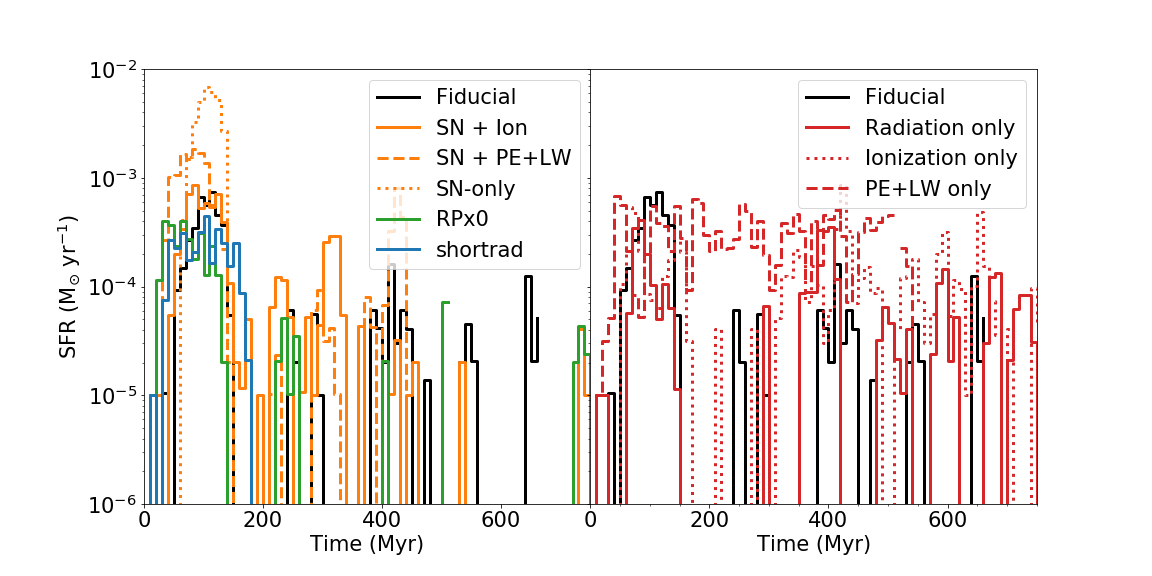
\includegraphics[width=0.98\linewidth]{figures/physics_comparison_sfr_2}
  \caption{The SFR in each of our runs, comparing those with SN feedback (left) to those without SN (right). The fiducial simulation, which includes all physics, is plotted in both panels (\fiducialstyle) for comparison.}
  \label{fig:SFR}
\end{figure*}

After the first 100~Myr, the differences between runs by the inclusion of SN feedback becomes obvious. Each of the SN-included runs (left panel) show various degrees of bursty star formation for the remainder of the simulation time, with lower average star formation rate than the ionization runs. The run with only PE heating and LW radiation, PE+LW (\pelwstyle), shows the most steady SFR, indicating that this feedback channel alone is capable of producing a self-regulating SFR in this galaxy, but not the bursty star formation that is seen with the inclusion of any other feedback channel. Ionization alone (\ionstyle) and the combined radiation run (\radstyle) both show burst star formation like the SN runs, but still have a higher average SFR and more consistent SF through the end of the simulation. The SN runs have progressively lower SFR and longer quiescent periods as each simulation proceeds.

\textbf{I may remove Shortrad and RP0 from these plots and save discussion of them for later... that way I can also show RP2 and RP5 better... all at once will be pretty cluttered (as if it isn't already)}

(\textbf{Maybe show summary table of comparison values? average SFR, average retention fractions, average outflow, etc.?... maybe do this in discussion... also show energy, mass, metal ejection efficiencies and laoding factors as per Li+Byran 2019}?

\subsection{Global Galaxy Properties}
\label{sec:galaxy properties}

In Figure~\ref{fig:properties} we compare the time evolution of the total \HI mass, stellar mass, H$_2$ mass fraction, and average ISM metallicity for each of our runs. The \HI mass in the fiducial simulation declines with time as stars form, radiation ionizes the ISM, and SN feedback drives significant mass loss. Interestingly the H$_2$ fraction increases significantly during this time, but, as shown in Paper~I, this is mostly due to the preferential retention of the cold, dense gas where the H$_2$ resides, rather than the generation of a significant amount of mass of molecular hydrogen. In the bottom right panel we show the evolution of only those metals self-consistently produced by stars formed in the simulation; the initial metal fraction for these species is 10$^{-20}$. In the fiducial run, the mean ISM metallicity remains well below what could be expected for a closed-box model (black, dashed). As discussed in Section~\ref{sec:outflows} this is due to the significant outflows generated by feedback in this galaxy. 

\begin{figure*}
  \centering
  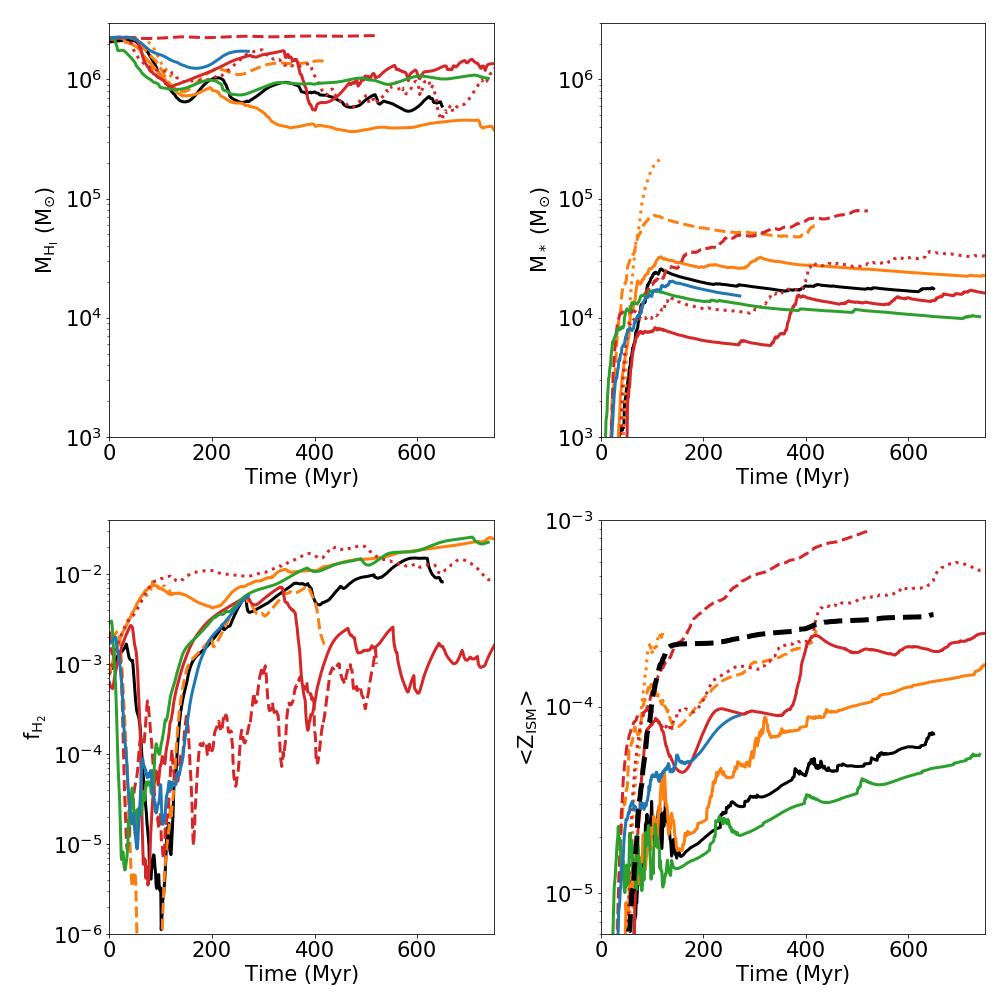
\includegraphics[width=0.98\linewidth]{figures/physics_comparison_masses}
  \caption{The evolution of four global galaxy properties for each of our simulations. Clockwise from top left: \HI mass, stellar mass, H$_2$ fraction, and mean ISM metallicity. $M_{\rm \HI}$ and $M_{*}$ have the same vertical axis limits for comparison of the stellar mass fraction between runs. The $<Z_{\rm ISM}>$ shown here only includes metals self-consistently produced by stars in this simulation (see text).
  \textbf{Include legend again?}}
  \label{fig:properties}
\end{figure*}

SN+Ion produces the lowest \HI mass of all of the runs. Compared to the fiducial simulation, this is likely due to the increase in stellar mass and increase in number of ionizing photons (\textbf{though maybe also outflows...check later}). Each of the other simulations have a higher \HI mass, in spite of the fact that most have higher total stellar masses. The common theme among these runs is the lack of ionizing radiation, which, along with outflows, is clearly important for regulating the neutral gas fraction of this galaxy. The importance of outflows in regulating the gas content can be seen by comparing the radiation only (\radstyle) run to the fiducial, which shows a similar total stellar mass but greater \HI content, and the ionization only run (\ionstyle) which has a stellar mass higher than both the fiducial and SN+Ion runs but a comparable \HI mass to the fiducial run. At the extreme, PE+LW radiation alone clearly is incapable of ionizing or removing any \HI from this galaxy, in spite of its comparatively high stellar mass. Interestingly, the total stellar mass for the SN+PE+LW run is similar to that with PE+LW alone -- further indicating that PE+LW are not significant sources of pre-SN feedback compared to ionizing radiation -- but has a lower \HI mass, likely due to SN-driven outflows. Wewill discuss outflows in more detail in Section~\ref{sec:outflows}.

\textbf{It may be worth exploring in more detail why the radiation run and ionization only runs have lower stellar masses for first few Myr than the fiducial.}

With the exception of the radiation (\radstyle) and PW+LW (\pelwstyle) runs, the molecular hydrogen fraction is quite similar throughout the galaxy's evolution. What is most clear from this plot is that stellar LW radiation is indeed important to consider if attempting to model the molecular gas content. The two runs without LW radiation (SN+Ion and ionization-only) show fewer fluctuations in the molecular gas content than the other runs, most obvious during the initial 100~Myr burst where the $H_2$ fractions drop dramatically for those runs with LW radiation. \textbf{not sure if need more here? also not sure if it would be better to plot H2 mass to remove the evolution of the denominator from the interpretation?}

Understandably, the differences in stellar mass evolution and gas content in these runs leads to a significant variation in the mean ISM metal fraction. The fiducial run 

\subsection{Evolution of Individual Metals}
\textit{Decide if this comes before or after outflow section}

As explored in \citep{Emerick2018b}, metals released into the ISM in core collapse supernova are ejected from the galaxy through outflows at a higher efficiency than metals from AGB winds. In addition, these same metals showed smaller gas-phase abundance variations -- pointing to more efficient mixing -- than elements from AGB winds. We explore how feedback affects these differences here.

\begin{figure*}
  \centering
  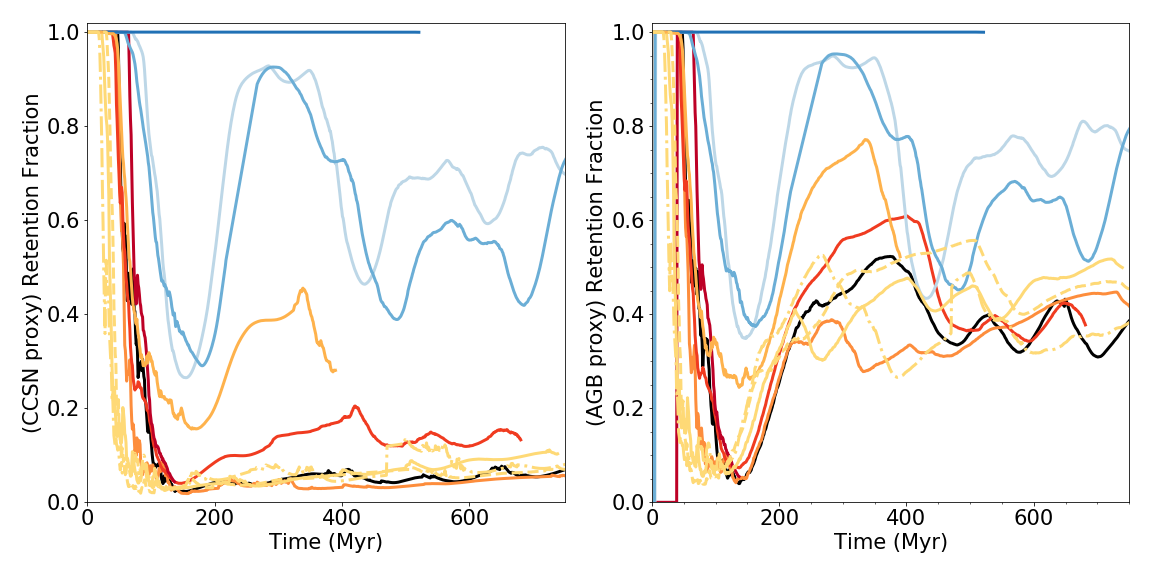
\includegraphics[width=0.95\linewidth]{figures/physics_comparison_retention}
  \caption{The retention fraction of CCSN elements (left, traced by O) and AGB elements (right, traced by Ba) in the disk of each galaxy as a function of time.}
  \label{fig:retention}
\end{figure*}

In Figure~\ref{fig:retention} we plot the fraction of metals produced that remain within the disk for a CCSN proxy (Oxygen, left) and an AGB enrichment proxy (Ba, right). The fiducial simulation shows a fairly consistent CCSN retention fraction of $\sim$5\% after the first 100~Myr. The AGB retention fraction drops during the first 100~Myr until the first AGB begin producing significant Ba; the retention fraction then grows and oscillates with the SFR, but remains around 40\%, significantly higher than that for CCSN elements. In general, runs with SN feedback show low CCSN element retention, yet that without ionizing radiation (SN+PE+LW) shows a larger retention fraction ($\sim$20\%). A similar picture is true for the AGB elements, where the SN-included runs show the lowest retention fractions. However, in all cases the AGB element retention fraction is higher than the SN element retention fraction. The runs without SN show nearly identical retention fractions for both elements. Interestingly, the two radiation runs with ionizing radiation show dramatic fluctuations in the retention fractions (\textbf{I'm assuming this is because the galaxy is "breathing" rather than having big outflows, and this is just the fluctuations of gas across the arbitrary disk boundary... check this...}) This is additional confirmation that this difference is due in large part to the difference in energetics between the SN and AGB events, as expected from the analysis in \cite{Emerick2020a}. 

\textit{I thought this would be a cool find if the CGM / halo retention fraction was different between hte two elements, but it appears not... Might still be interesting to have this here, but maybe not worth a figure:} Although the mass of this galaxy is likely too low to observe the metal content of its circumgalactic medium, where the metals end up beyond the disk of the galaxy may also be an important discriminator between feedback models. We explore this here to motivate future study in more massive dwarf galaxies. We find that the fraction of metals in the CGM for CCSN is initially large after the first burst of star formation ($\sim$80-90\%) for all SN runs, but gradually declines to $\sim$20-30\% by the end of the simulation. Since this lost mass is not being re-accreted into the ISM, it is being lost beyond the halo. Although AGB elements show significantly different dsk retention fractions, the CGM fractions are very similar to the CCSN elements. Whatever AGB elements do end up in the halo were carried out through the same processes as the CCSN elements, leading to the very similar evolution in the CGM. % if the fractions were different that wouldve been cool

%In Figure~\ref{fig:CGM} we plot the gravitationally bound 

\begin{figure*}
  \centering
  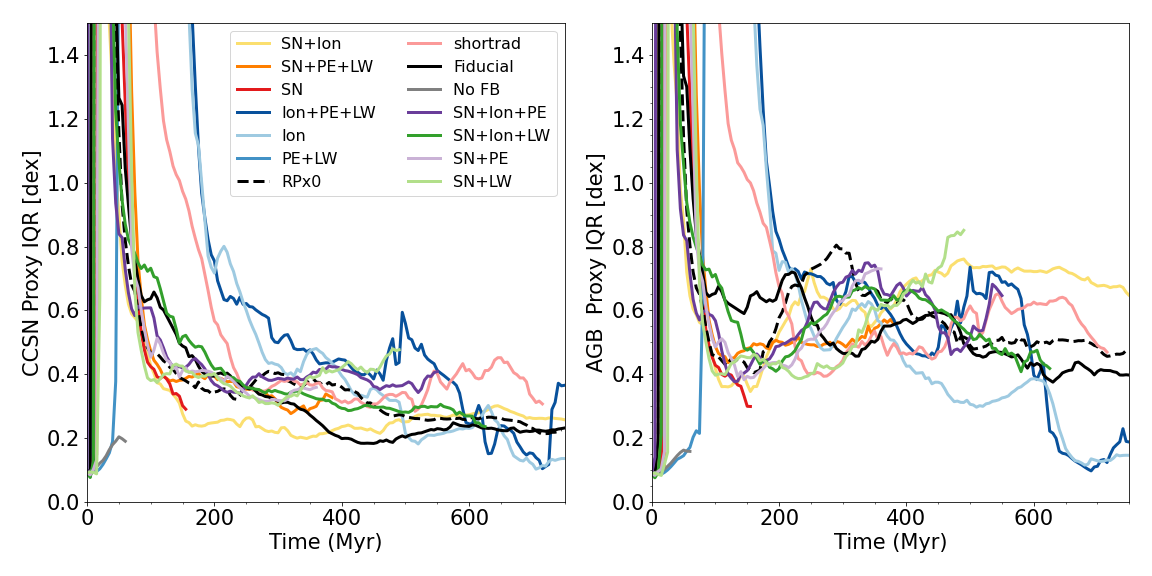
\includegraphics[width=0.95\linewidth]{figures/physics_comparison_IQR}
  \caption{A comparison of the evolution of the inner quartile range (IQR) of the gas-phase abundances of CCSN elements (left, traced by O) and AGB wind elements (right, traced by Ba) in the cold ISM (\textbf{give n,T bounds}). Run Pe+LW (\pelwstyle) remains well above the vertical bounds for the duration of the simulation, and is omitted for clarity (see text).}
  \label{fig:mixing}
\end{figure*}

Finally, we explore the metal mixing differences between these runs and these two elements in Figure~\ref{fig:mixing}. We compare the inner quartile range (IQR) abundance spread of the cold gas for O, the CCSN element proxy, and Ba, the AGB element proxy, for each run. In the fiducial simulation, the CCSN elements show a declining spread throughout the evolution, reaching an IQR of $\sim$0.25 dex by the end of the simulation time. As was seen in the retention fraction, the AGB elements follow the same evolution until first produced by AGB, at which point the width rises significantly, to around 0.7~dex, and remaining well above the CCSN elements until the end of the simulation. All of the simulations including SN feedback show very similar general trends and final IQR values; the notable exception to this is the significantly larger rise in IQR in the AGB elements for run SN+Ion (\textbf{not sure why... need to think...}). The comparison to the radiation only runs shows the importance that hot-phase mixing has on the evolution of these elements. While the runs with SN hit a roughly consistent IQR after the first $\sim$150~Myr, the runs without SNe take a little more than twice as long to reach this point. This is in spite of the fact that the radiation-only runs have a higher global SFR with more continual and uniformly distributed (\textbf{check this}) enrichment that should allow for more rapid homogenization. However, the radiation only runs do not have SN depositing their elements first in a volume-filling hot phase, which is necessary for rapid mixing over the whole galaxy. However, ionizing radiation generates sufficiently warm / hot gas to increasing the mixing timescales of these elements. Not shown in either panel for clarity is run PE+LW, which exhibits mixing timescales on order of the dynamical time of this galaxy ($\sim$1~Gyr). This run has a gradually declining IQR like the rest of the simulations, but still has an exceedingly large IQR of 5~dex in both elements by the end of the simulation.

Since SN and AGB winds have the same injection energy in the radiation only runs, they exhibit very similar abundance spreads. This suggests that, not only is the mean abundance of individual elements an important discriminator between feedback models, but also the scatter in individual abundances can contain information about the stellar feedback that drives metal mixing in the ISM.

\subsection{Outflows}
\textbf{Might move this before metal retention plots. Show mass outflow and metal outflow rates (and loading?) at 0.1 Rvir and 1.0 Rvir (maybe). Maybe don't show energy loading and save that for just the time-averaged single point discussion later}. 

\subsection{Multi-Phase ISM}
\textbf{Discuss properties of multi-phase ISM here. Possibly show mass and volume fractions, but possibly more interesting / pretty to just show a large panel of phase diagrams. Both would likely be too much. Would be nice if comparison made it clear what features were cause by what process}.




\section{Discussion}

\textit{Maybe put Li+Byran2019 comparison values here?}

Summarize this feedback exploration in terms of both what physics is important to model but ALSO what are the general "modes" of feedback (i.e. what affects certain properties the most but also HOW each thing operates). 


\section{Conclusion}
If separate from above?

%\acknowledgments
\section*{Acknowledgments} AE was supported by ??????. \textbf{CHECK IF CORRECT:} GLB acknowledges support from NSF grants AST-1615955 and OAC-1835509 and NASA grant NNX15AB20G. M-MML was partly supported by NSF grant AST18-15461. We gratefully recognize computational resources provided by NSF XSEDE through grant number TGMCA99S024, the NASA High-End Computing Program through the NASA Advanced Supercomputing Division at Ames Research Center, Columbia University, and the Flatiron Institute. This work made significant use of many open source software packages. These are products of collaborative effort by many independent developers from numerous institutions around the world. Their commitment to open science has helped make this work possible. 

%mm many citations from citebay.com.  Don't know what to cite for deepdish, so just put a placeholder in.
\software{\textsc{yt} \citep{yt}, \textsc{Enzo} \citep{Enzo2014}, \textsc{Grackle} \citep{GrackleMethod}, \textsc{Python} \citep{VanRossum1995python}, \textsc{IPython} \citep{perez2007ipython}, \textsc{NumPy} \citep{oliphant2006guide}, \textsc{SciPy} \citep{SciPy}, \textsc{Matplotlib} \citep{hunter2007matplotlib}, \textsc{HDF5} \citep{Fortner1998HDF,Koranne2011}, \textsc{h5py} \citep{h5py}, \textsc{Astropy} \citep{astropy:2013,astropy:2018}, \textsc{Cloudy} \citep{Cloudy2013}, and \textsc{deepdish}}

%\begin{figure*}
%  \centering
%  \includegraphics[width=0.45\linewidth]{figures/combined_CGM_average_evolution}
%  \includegraphics[width=0.45\linewidth]{figures/combined_CNM_average_evolution}\\
%  \includegraphics[width=0.45\linewidth]{figures/combined_CNM_average_mean-median}
%   \includegraphics[width=0.45\linewidth]{figures/combined_CNM_average_rms}
%  \caption{The same as Figure~\ref{fig:CGM_CNM} and Figure~\ref{fig:mean-median}, but comparing across both sets of runs with different SFRs. Line color corresponds to a fixed enrichment energy event, while the solid lines correspond to the higher SFR runs discussed throughout this work, and the dashed lines the lower SFR runs. See text for more details.}
%  \label{fig:SFR_comparison_CGM_CNM}
%\end{figure*}


%************* APPENDICES ************************%

%\section*{Acknowledgments}

%\clearpage
%\appendix - Liklely DO NOT use this command
%\setcounter{section}{0}%
%\renewcommand\thesection{\thechapter.\Alph{section}}
%\counterwithin{figure}{section}

%
% Place appendix here
%


\bibliographystyle{yahapj}
\bibliography{refs}

\end{document}
